\documentclass[10pt,a4paper]{article}

\usepackage[utf8]{inputenc}
\usepackage[T1]{fontenc}
\usepackage[brazil]{babel}
\usepackage{helvet}
\renewcommand{\familydefault}{\sfdefault}
\usepackage[top=18mm,bottom=18mm,left=16mm,right=16mm]{geometry}
\usepackage{xcolor}
\usepackage{graphicx}
\usepackage{booktabs}
\usepackage{tabularx}
\usepackage{array}
\usepackage{colortbl}
\usepackage{fancyhdr}
\usepackage{lastpage}
\usepackage{hyperref}
\usepackage{parskip}

% Paleta Oficial - Jornal Economico do Tocantins
\definecolor{azulto}{HTML}{0F2537}
\definecolor{douradoto}{HTML}{C8942B}
\definecolor{cinzafundo}{HTML}{F4F6F9}
\definecolor{cinzatexto}{HTML}{2C353D}
\definecolor{cinzasuave}{HTML}{6C757D}
\definecolor{vermelhoalerta}{HTML}{D85C5C}
\definecolor{borda}{HTML}{DEE2E6}

\hypersetup{
    colorlinks=true,
    linkcolor=azulto,
    urlcolor=douradoto,
    pdftitle={Balança comercial do Tocantins mantém superávit robusto no mês puxada pelo complexo soja e carnes},
    pdfauthor={Lorenzo Costa e Equipe | Jornal Econômico do Tocantins}
}

\setlength{\parindent}{0pt}
\setlength{\parskip}{6pt}
\renewcommand{\arraystretch}{1.28}

% Cabecalho e Rodape Padronizados
\pagestyle{fancy}
\fancyhf{}
\renewcommand{\headrulewidth}{0pt}
\renewcommand{\footrulewidth}{0.6pt}
\renewcommand{\footrule}{\hbox to\headwidth{\color{douradoto}\leaders\hrule height \footrulewidth\hfill}}

\fancyfoot[L]{\footnotesize\textcolor{cinzasuave}{\textbf{Jornal Econômico do Tocantins} $\bullet$ BOLETIM FLASH • COMÉRCIO EXTERIOR $\bullet$ Outubro/2026}}
\fancyfoot[R]{\footnotesize\textcolor{cinzasuave}{Página \thepage\ de \pageref{LastPage}}}

% Comando para Titulos de Secao Padronizados
\newcommand{\secaojornal}[1]{%
  \vspace{6pt}%
  {\noindent\colorbox{azulto}{%
    \parbox{\dimexpr\textwidth-2\fboxsep\relax}{%
      \vspace{3pt}\hspace{4pt}\textcolor{douradoto}{\rule{7pt}{7pt}}\hspace{6pt}%
      \textcolor{white}{\textbf{\normalsize \MakeUppercase{#1}}}\vspace{3pt}%
    }%
  }}%
  \vspace{4pt}%
}

\begin{document}
\color{cinzatexto}

% ==============================================================================
% FAIXA INSTITUCIONAL DE CABECALHO (AZUL MARINHO + DOURADO)
% ==============================================================================
\noindent\colorbox{azulto}{%
  \parbox{\dimexpr\textwidth-2\fboxsep\relax}{%
    \vspace{6pt}%
    \begin{tabularx}{\linewidth}{@{}X r@{}}
      {\fontsize{15}{18}\selectfont\textbf{\textcolor{white}{JORNAL ECONÔMICO DO TOCANTINS}}} &
      \colorbox{douradoto}{\textbf{\footnotesize\textcolor{azulto}{\hspace{4pt}BOLETIM FLASH • COMÉRCIO EXTERIOR\hspace{4pt}}}} \\[4pt]
      {\footnotesize\textcolor{douradoto}{\textbf{Núcleo de Inteligência e Conjuntura Econômica Regional}}} &
      {\footnotesize\textcolor{white}{Referência: \textbf{Outubro/2026} $\vert$ Publicado em 30/10/2026}}
    \end{tabularx}%
    \vspace{4pt}%
  }%
}\\[-2pt]
\noindent{\color{douradoto}\rule{\textwidth}{2.5pt}}

\vspace{6pt}

% ==============================================================================
% TITULO, SUBTITULO E AUTORIA
% ==============================================================================
{\fontsize{16}{20}\selectfont\textbf{\textcolor{azulto}{Balança comercial do Tocantins mantém superávit robusto no mês puxada pelo complexo soja e carnes}}}\\[4pt]
{\normalsize\textcolor{cinzasuave}{Embarques para o mercado asiático sustentam geração líquida de divisas e compensam importação de fertilizantes}}\\[4pt]
{\footnotesize\textcolor{azulto}{\textbf{Análise e Redação:}} \textcolor{cinzatexto}{Lorenzo Costa e Equipe | Jornal Econômico do Tocantins} \hfill \textcolor{azulto}{\textbf{Base Oficial:}} \textcolor{cinzatexto}{Comex Stat / MDIC}}

\vspace{2pt}

% Destaque Executivo (Resumo em Caixa)
\noindent\fcolorbox{douradoto}{cinzafundo}{%
  \parbox{\dimexpr\textwidth-2\fboxsep-2\fboxrule\relax}{%
    \vspace{3pt}%
    \textbf{\textcolor{azulto}{Síntese Executiva:}} Com exportações acumuladas de US\$ 2,54 bilhões e saldo positivo de US\$ 2,06 bilhões, o setor externo tocantinense registra índice de cobertura de 5,3 vezes sobre as compras externas.%
    \vspace{3pt}%
  }%
}

\vspace{4pt}

% ==============================================================================
% CAIXAS DE INDICADORES-CHAVE (GERADAS AUTOMATICAMENTE PELO R)
% ==============================================================================
\noindent\colorbox{azulto}{\parbox[t][1.32cm][c]{0.225\textwidth}{\centering\scriptsize\textcolor{white}{\textbf{Exportações (FOB)}}\\[3pt]{\large\textbf{\textcolor{douradoto}{US\$ 200,89 Mi}}}}}\hfill\colorbox{azulto}{\parbox[t][1.32cm][c]{0.225\textwidth}{\centering\scriptsize\textcolor{white}{\textbf{Importações (FOB)}}\\[3pt]{\large\textbf{\textcolor{douradoto}{US\$ 63,95 Mi}}}}}\hfill\colorbox{azulto}{\parbox[t][1.32cm][c]{0.225\textwidth}{\centering\scriptsize\textcolor{white}{\textbf{Saldo Comercial}}\\[3pt]{\large\textbf{\textcolor{douradoto}{+ US\$ 136,94 Mi}}}}}\hfill\colorbox{azulto}{\parbox[t][1.32cm][c]{0.225\textwidth}{\centering\scriptsize\textcolor{white}{\textbf{Corrente Total}}\\[3pt]{\large\textbf{\textcolor{douradoto}{US\$ 264,84 Mi}}}}}
\vspace{5pt}


% ==============================================================================
% SECAO 1: ESTATISTICA DESCRITIVA AUTOMATIZADA E EVIDENCIA EMPIRICA
% ==============================================================================
\secaojornal{1. Panorama Estatístico e Resultados do Período (Síntese Automatizada)}

No período de referência (Outubro/2026), a corrente total de comércio exterior do Estado do Tocantins (soma das exportações e importações) atingiu US\$ 264,84 milhões. As vendas externas somaram US\$ 200,89 milhões (US\$ 200,89 Mi), ao passo que as aquisições de produtos estrangeiros totalizaram US\$ 63,95 milhões (US\$ 63,95 Mi). Como resultado, a balança comercial tocantinense apresentou expressivo superávit comercial e acumulou geração líquida positiva de divisas da ordem de US\$ 136,94 milhões (+ US\$ 136,94 Mi), com índice de cobertura de 3,1x (exportações equivalentes a 3,1 vezes o valor importado).

\vspace{4pt}

Na decomposição setorial da pauta exportadora por posição SH4, o desempenho foi puxado por Carnes de animais da espécie bovina, congeladas, que movimentou US\$ 50,28 milhões (42,2\% do top 3 exportador), seguido por Soja, mesmo triturada com US\$ 36,35 milhões (30,5\%). Pela ótica das importações, a demanda estadual concentrou-se em Adubos (fertilizantes) azotados (US\$ 34,82 milhões, ou 76,9\% dos principais itens), refletindo a estrutura de custos de insumos produtivos. Geograficamente, China consolidou-se como o principal destino individual das exportações estaduais (US\$ 46,97 milhões, respondendo por 23,4\% do total exportado), enquanto China liderou a origem das compras externas (US\$ 15,98 milhões).

\vspace{4pt}

\begin{center}
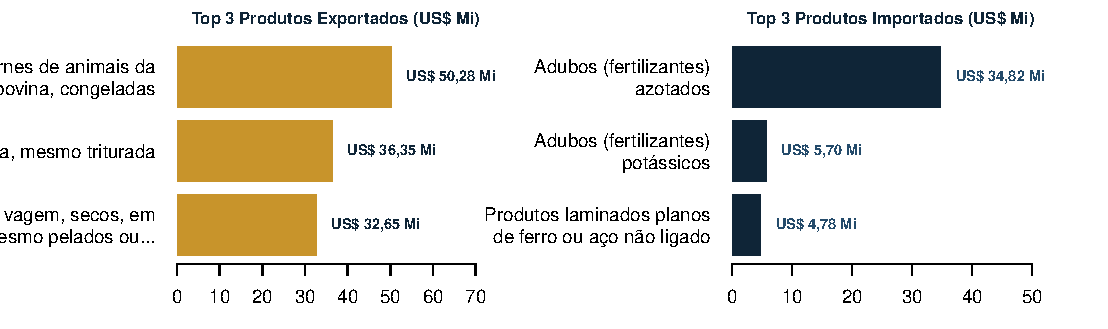
\includegraphics[width=\textwidth]{boletins/build/fig_2026_10_flash_comex.pdf}
\end{center}
\vspace{1pt}
\noindent\begin{minipage}{\textwidth}
{\footnotesize
\noindent\textbf{\textcolor{azulto}{Tabela 1 — Principais Parceiros Comerciais do Tocantins (Destinos de Exportação e Origens de Importação)}}\\[2pt]
\begin{tabularx}{\linewidth}{@{}X r r @{\hspace{16pt}} X r r@{}}
\toprule
\rowcolor{azulto} \textcolor{white}{\textbf{Destino (Exportação)}} & \textcolor{white}{\textbf{US\$ Mi}} & \textcolor{white}{\textbf{Part. (\%)}} & \textcolor{white}{\textbf{Origem (Importação)}} & \textcolor{white}{\textbf{US\$ Mi}} & \textcolor{white}{\textbf{Part. (\%)}} \\
\midrule
China & 46,97 & 23,4\% & China & 15,98 & 25,0\% \\
Índia & 33,59 & 16,7\% & Nigéria & 14,93 & 23,3\% \\
Canadá & 16,57 & 8,2\% & Venezuela & 14,67 & 22,9\% \\
Egito & 16,18 & 8,1\% & Canadá & 5,71 & 8,9\% \\
Espanha & 10,32 & 5,1\% & Estados Unidos & 4,48 & 7,0\% \\
Suíça & 8,20 & 4,1\% & Vietnã & 3,90 & 6,1\% \\
\bottomrule
\end{tabularx}
}
\end{minipage}
\vspace{2pt}


% ==============================================================================
% SECAO 2: ANALISE HUMANA E INTERPRETACAO DA EQUIPE
% ==============================================================================
\secaojornal{2. Análise de Conjuntura e Leitura da Equipe}

O resultado mensal da balança comercial do Tocantins reforça a posição estratégica do Estado como plataforma agroexportadora da região Norte. O desempenho das vendas externas segue ancorado na competitividade da soja em grãos e da carne bovina in natura, que encontraram janelas favoráveis de embarque nos portos do Arco Norte e demanda firme dos compradores asiáticos.

\vspace{4pt}

Pelo lado das importações, o desembolso de US\$ 480 milhões reflete o calendário de aquisição de adubos, fertilizantes e defensivos agrícolas para o plantio da safra. Esse movimento é típico de economias em expansão produtiva, nas quais a compra externa de insumos antecede a geração de excedentes exportáveis nos meses subsequentes.

% ==============================================================================
% SECAO 3: PERSPECTIVAS E CENARIOS
% ==============================================================================
\secaojornal{3. Perspectivas e Cenários}

Para os próximos meses, a expectativa é de manutenção do saldo comercial amplamente superavitário, favorecido pela taxa de câmbio em patamar competitivo em reais e pelo escoamento dos estoques estaduais de milho e proteína animal.

\vfill
\noindent{\color{borda}\rule{\textwidth}{0.5pt}}\\[-2pt]
{\scriptsize\textcolor{cinzasuave}{\textbf{Nota Metodológica e Fontes:} Ministério do Desenvolvimento, Indústria, Comércio e Serviços (Comex Stat / MDIC). Elaboração: Jornal Econômico do Tocantins. Documento gerado de forma automatizada pelo Sistema Editorial Híbrido (R + LaTeX) do Jornal Econômico do Tocantins.}}

\end{document}
